\section{Summary}

\begin{frame}{What Have We Learned?}
    \begin{center}
        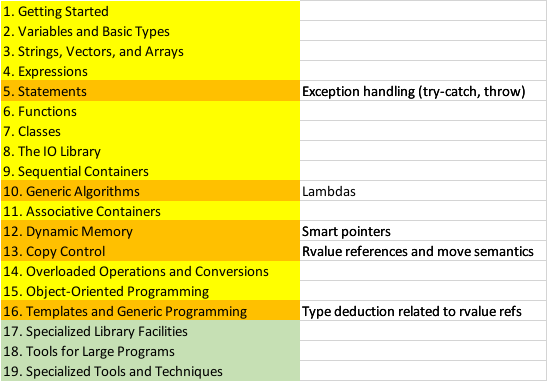
\includegraphics[width = 0.95\textwidth]{img/contents.png}
    \end{center}
\end{frame}

\begin{frame}
    \begin{center}
        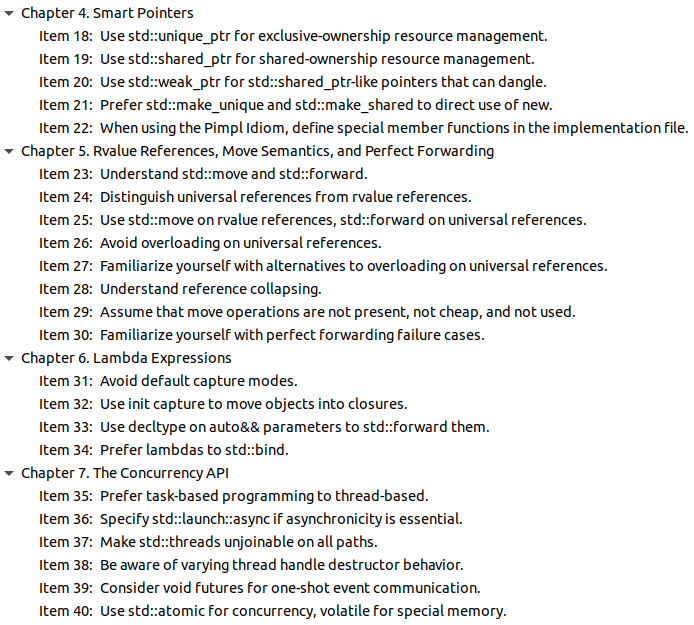
\includegraphics[width=0.85\textwidth]{img/effectivemodern.png}
    \end{center}
\end{frame}

\begin{frame}{Exception Handling}
    \begin{itemize}
        \item \ttt{try-catch}, \ttt{throw} and the exception classes defined in the standard library
        \item \textit{Effective C++} Item 8, 25, 29.
    \end{itemize}
\end{frame}

\begin{frame}{Concurrency}
    Multi-threading in C++: \ttt{<thread>}, \ttt{<future>}, \dots (since C++11)\\
    Play with them in CS110!
\end{frame}

\begin{frame}[fragile]{The Boost Library}
    A collection of high quality, open source, platform- and compiler-independent libraries. \url{http://boost.org}
    \begin{itemize}
        \item Lambda: (Unlike C++11 lambda)
        \begin{cpp}
std::for_each(v.begin(), v.end(),
            std::cout << _1 * 2 + 10 << '\n');
        \end{cpp}
        \item Template metaprogramming library (mpl)
        \item Math and numerics
        \item Inter-language support (e.g. boost python)
        \item Memory management
        \item Graph library
        \item \dots\dots
    \end{itemize}
\end{frame}